\documentclass[tiny]{corsage}

\usepackage[spanish]{babel}
\usepackage[T1]{fontenc}
\usepackage[utf8]{inputenc}
\usepackage{amsmath}
\usepackage{amssymb}
\usepackage{amsthm}
\usepackage{hyperref}
\usepackage{indentfirst}
\usepackage{microtype}
\usepackage{minted}
\usepackage{tcolorbox}
\usepackage{xcolor}

\newcommand{\R}{\mathbb{R}}
\newcommand{\Tri}{\text{Tri}}
\newcommand{\segment}[1]{\overline{#1}}
\newcommand{\cost}[1]{\text{cost}(#1)}

\theoremstyle{plain}
\newtheorem{theorem}{Teorema}

\theoremstyle{definition}
\newtheorem{defthm}{Definición}

\definecolor{definition-line}{HTML}{FF4040}
\definecolor{definition-background}{HTML}{FFE0E0}

\hypersetup{
    pdftitle={3ds min 2026},
    pdfauthor={Autodesc}
}

\setminted{
	encoding=utf8,
	ignorelexererrors=true
}

\makeatletter
\newcommand*{\@doendeq}{%
	\everypar{{\setbox\z@\lastbox}\everypar{}}%
}
\makeatother

\newcommand{\rest}{%
	\par
	\vspace{0.5\parskip}%
	\begin{center}%
		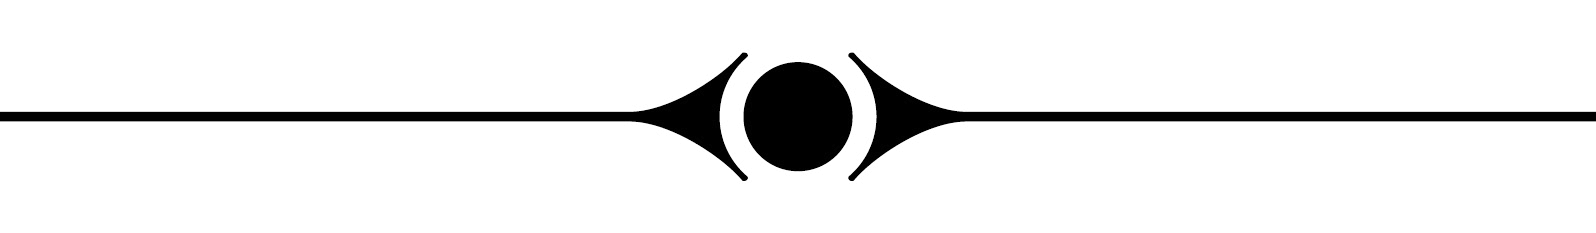
\includegraphics[width=0.2\linewidth]{rest}%
	\end{center}%
	\vspace{-\parskip}%
	\ignorespacesafterend\par\noindent\aftergroup%
}

\newcommand{\pant}{%
	\par
	\vspace{0.5\parskip}%
	\begin{center}%
		\centerline{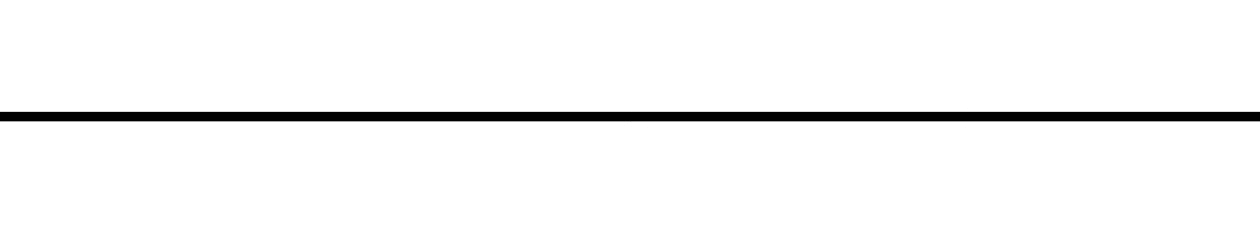
\includegraphics[width=0.15\linewidth]{pant}}
	\end{center}%
	\vspace{-\baselineskip}%
	\par\ignorespacesafterend\noindent\aftergroup%
}

\makeatletter
\newenvironment{definition}{%
	\begin{tcolorbox}[
		left skip=0.5cm,
		right skip=0.5cm,
		left=8pt,
		right=8pt,
		top=3\parskip,
		bottom=0.25\parskip,
		colback=definition-background,
		colframe=definition-line,
		boxrule=0pt,
		leftrule=4pt,
		sharp corners=all
	]%
	\begin{defthm}%
}{%
	\end{defthm}%
	\end{tcolorbox}%
	\ignorespacesafterend\par\noindent\aftergroup\@doendeq%
}

\makeatother

\begin{document}
\section{Definición del enunciado}
	Considere un polígono convexo $P = \langle v_0, v_1, v_2, \dots, v_{n - 1} \rangle$ con $n$ lados $\segment{v_0v_1}$, $\segment{v_1,v_2}$, $\dots$, $\segment{v_{n - 1}v_n}$,  donde $v_n = v_0$.  Dados dos vértices no adyacentes $v_i$ y $v_j$, llamamos al segmento $\segment{v_iv_j}$ una \emph{cuerda} del polígono.

	Una \emph{triangulación} del polígono $P$ es un conjunto $T$ que lo divide en triángulos disjuntos.  En una triangulación, las cuerdas no se intersecan salvo en los vértices, y el conjunto $T$ es maximal:  Cada cuerda no perteneciente a $T$ interseca alguna cuerda de $T$.  Los lados de los triángulos producidos por la triangulación son o bien cuerdas pertenecientes a $T$ o lados del polígono.  Dado un mismo polígono, existen múltiples formas de triangularlo.

	\begin{definition}	
		Dados un polígono $P = \langle v_0, v_1, v_2, \dots, v_{n - 1} \rangle$ y una función peso definida sobre los triángulos formados por una triangulación $w: \Delta(v_iv_jv_k) \to \R$, el \emph{problema de la triangulación óptima} consiste en encontrar una triangulación que minimice la suma de los pesos de todos los triángulos pertenecientes a la triangulación.
		\label{def-tri}
	\end{definition}
	
	Proponemos para este trabajo usar la siguiente función peso, que corresponde a calcular el perímetro del triángulo:
	\begin{equation}
		w(\Delta{u, v, w}) = \left | \segment{v_iv_j} \middle | + \middle | \segment{v_jv_k} \middle | + \middle | \segment{v_kv_i} \right |
		\label{fn-w}
	\end{equation}

	Dada una cuerda $\segment{v_iv_j}$ sobre el polígono $P$, quedan trazados dos \emph{subpolígonos} $P_{i, j} = \langle v_i, v_{i + 1}, v_{i + 2}, \dots, v_j \rangle$ y $P_{j, i} = \langle v_j, v_{j + 1}, v_{j + 2}, \dots, v_i \rangle$.  Nuestro problema es encontrar, dado un polígono convexo $P$ con $n$ lados y una función peso $w$:
	\begin{equation}
		\mathbb{S} = \min{\left \{ \sum_{\Delta \in T}{w(\Delta)} \ \middle | \  T \in \Tri(P) \right \}}
		\label{def-sol}
	\end{equation}

	De donde $\Tri(P)$ es el conjunto de todas las posibles triangulaciones para el polígono $P$.

\section{Solución óptima}
	La solución óptima para computar este problema nace a partir del siguiente Teorema:

	\begin{theorem}[Subestructura óptima]
		La triangulación óptima de un polígono convexo $P$ entre los vértices $i$, y $j$ debe contener las triangulaciones óptimas para los subpolígonos $P_{i,k}$ y $P_{k,j}$ para algún vértice $k$ intermedio.
		\label{thm-opt}
	\end{theorem}

	\begin{proof}
		La triangulación óptima de un polígono $P_{i,j}$ incluye por al menos un triángulo $\Delta(v_i, v_k, v_j)$ que lo divide en dos subpolígonos $P_{i,k}$ y $P_{k,j}$.  Si alguna de las triangulaciones cualquiera de los dos subpolígonos no es óptima, se podría reemplazarla por una óptima y obtener un mejor resultado global, contradiciendo la optimalidad.
	\end{proof}

	El Teorema \ref{thm-opt} indica que la triangulación óptima se compone directamente de las triangulaciones óptimas para de los dos subpolígonos determinados tras elegir un vértice $k$.  Nos proponemos ahora a encontrar una expresión general $\cost{i, j}$ para encontrar el costo de la triangulación óptima para un polígono $P$ entre $i$ y $j$.

	Sea $N = 1 + j - i$ la cantidad de vértices de $P$, resulta:
	\begin{itemize}
		\item \textbf{Si $N < 3$}, no tenemos suficientes vértices para formar ningún triángulo.  Por lo tanto, el costo de la triangulación debe ser cero.  (Definición \ref{def-tri})
		\item \textbf{Si $N = 3$}, hay exactamente un sólo triángulo que se puede formar con estos vertices, y por lo tanto, el costo de la triangulación será igual a $w(\Delta{v_i,v_{i+1},v_j})$.
		\item \textbf{Si $N > 3$}, hay más de una forma de triangular este polígono, por lo tanto, debemos elegir aquella con el menor costo.  Para cualquier $k \in [i + 1; j - 1]$, podemos trazar el triángulo $\Delta(v_i,v_k,v_j)$ que separa además a $P$ en dos subpolígonos $P_{i,k}$ y $P_{k,j}$.  Estos polígonos tienen $N_1 = 1 + k - i$ y $N_2 = 1 + j - k$ vértices respectivamente.

			Dado que $i < k < j$, y que $N > 3$, ambos subpolígonos deben tener como mínimo 2 vértices, y a lo sumo uno de ellos tendrá $N - 1$ vértices.  Por lo tanto, se puede aplicar la Hipótesis Inductiva para afirmar que $\cost{i, k}$ y $\cost{k, j}$ representan los costos mínimos de las triangulaciones óptimas de ambos subpolígonos.

			Ahora, según el Teorema \ref{thm-opt}, sabemos que el costo de la triangulación óptima entre $i$ y $j$ tendrá que ser:
			\[ \cost{i, j} = \min_{i < k < j}{\left [ \cost{i, k} + w(\Delta{v_iv_kv_j}) + \cost{k, j} \right ]} \]
	\end{itemize}

	Unificando los tres casos resulta:
	\begin{equation}
		\cost{i, j} = \left \{ \begin{array}{ll}
			0 & \text{si } j - i < 2 \\
			w(\Delta{v_iv_{i + 1}v_j}) & \text{si } j - i = 2 \\
			\cost{i, j} = \displaystyle\min_{i < k < j}{\left [ \cost{i, k} + w(\Delta{v_iv_kv_j}) + \cost{k, j} \right ]} & \text{de otro modo}
		\end{array}\right .
		\label{def-cost}
	\end{equation}

	Nótese que esta expresión es muy recursiva:  Para valores distintos de $k$ se llegará a consultar el costo de triangulación óptima de los mismos subpolígonos---en especial cuando estos tienen pocos vértices.  Para acelarar fuertemente la velocidad de la implementación de este algoritmo, se podría emplear \emph{programación dinámica}, y guardar el resultado de cada llamada en una caché, así la próxima vez que se quiera obtener el costo de triangulizar ese mismo polígono se evite realizar todos esos cálculos redundantes.

	Habiendo encontrado una expresión general para la función cost, podemos ahora calcular $\mathbb{S}$.  Dado un polígono $P$ con $N$ vértices, la \emph{solución al problema de la triangulación óptima} para este polígono, según la Hipótesis Inductiva, se obtiene:
	\[ \mathbb{S} = \cost{0, N - 1}\]

\section{Guía de implementación}
	A modo de ejemplo, proponemos una implementación en Haskell de un programa que calcula el costo de la triangulación óptima para un polígono convexo.  Para representar un polígono, decidimos utilizar \texttt{Data.Array} en lugar de una lista o un mapa debido a su acceso en tiempo constante.

	\begin{minted}{haskell}
import qualified Data.Array ((!))
import qualified Data.Map.Strict as M
import Control.Monad (replicateM)
import Data.Array hiding ((!))
import Data.Foldable (minimumBy)
import Data.List (sortOn, foldl')
import Data.Map.Strict ((!))
import Data.Ord (comparing)
import System.Process

-- | ¡claro que sí!
(¡) :: Ix i => Array i e -> i -> e
(¡) = (Data.Array.!)

infinity :: Float
infinity = 1.0 / 0.0

data Vertex = Vertex !Float !Float deriving (Eq, Show)

distance :: Vertex -> Vertex -> Float
distance (Vertex x0 y0) (Vertex x1 y1) = sqrt $ sq (x0 - x1) + sq (y0 - y1)
	where sq x = x * x

weight :: Vertex -> Vertex -> Vertex -> Float
weight v0 v1 v2 = distance v0 v1 + distance v1 v2 + distance v2 v0

type Elements = Array Int Vertex

newtype Poly = Poly Elements deriving (Eq, Show)
	\end{minted}

	Adicionalmente, proponemos dos simples funciones para generar polígonos convexos regulares e irregulares dado un radio y la cantidad de vértices.  Notamos que, como el módulo \texttt{System.Random} ya no está presente en el paquete \texttt{base} y para evitar agregar paquetes de tercero, recurrimos a una solución intencionalmente estrambótica que utiliza Python para generar números aleatoreos:

	\begin{minted}{haskell}
regular :: Float -> Int -> Poly
regular r n = Poly . listArray (0, n - 1)
	        $ map (point . angle . fromIntegral) [1..n]
        where point a = Vertex (r * cos a) (r * sin a)
              angle x = x * ((2 * pi) / fromIntegral n)

randomFloat :: Float -> Float -> IO Float
randomFloat a b = read <$> readProcess "python3" ["-c",
        "import random; print(random.uniform("
                ++ show a ++ ", " ++ show b ++ "))"] ""

irregular :: Float -> Int -> IO Poly
irregular r p = do
        angles <- replicateM p (randomFloat 0 (2 * pi))
        let points = map (\a -> Vertex (r * cos a) (r * sin a)) angles
        pure . Poly . listArray (0, p - 1) $
                sortOn (\backslash(Vertex x y) -> atan2 y x) points
	\end{minted}

	Para la caché y el uso de programación dinámica, sí optamos por utilizar \texttt{Data.Map}, dado que es más sencillo de modificar que un Array.  Esto cambia la complejidad asintótica del algoritmo, dado que no permite lectura y escritura en tiempo constante, pero facilita mucho la comprensión del código.
	\begin{minted}{haskell}
type Cache = M.Map (Int, Int) Float
	\end{minted}

	Ahora, podemos implementar la función \texttt{cost}.  Su implementación es casi idéntica a lo propuesto en la Ecuación \ref{def-cost}, con dos casos agregados:  Primero---y esto no es necesario, pero puede ser más elegante que tirar un error---proponemos que la función cost está definida cuando $i > j$, y que vale lo mismo que $\cost{j, i}$.  De estar usando algo como LiquidHaskell, en donde se podría asertar que $i < j$ analíticamente, no hubieramos optado por hacer esto.

	El segundo caso agregado, en cambio, simplemente corresponde a la programación dinámica:  Debemos consultar si este es un subproblema que ya hemos resuelto para evitar resolverlodos veces.

	\begin{minted}{haskell}
cost :: Cache -> Elements -> Int -> Int -> (Cache, Float)
cost !cache vs !i !j
        | j < i = cost cache vs j i
        | j - i <  2 = (cache, 0.0)
        | j - i == 2 = (cache, weight (vs ¡ i) (vs ¡ (i + 1)) (vs ¡ (i + 2)))
        | M.member (i, j) cache = (cache, cache ! (i, j))
        | otherwise = foldl' minK (cache, infinity) ks
       where general cache' k =
                let (!cache'', cLeft) = cost cache' vs i k
                    (cache''', cRight) = cost cache'' vs k j
                    w = weight (vs ¡ i) (vs ¡ k) (vs ¡ j) + cLeft + cRight
                 in (M.insert (i, j) w cache''', w)
             minK (!cache', minW) k =
                let (cache'', w) = general cache' k
                 in (cache'', min w minW)
             ks = [i + 1..j - 1]
	\end{minted}

	El caso general---como sabemos que hay al menos dos elementos en \texttt{ks}---iterará mediante todas las opciones con \texttt{foldl'}.  La función \texttt{minK} en el fold se encarga de recolectar todos los aportes de memoización realizados por las llamadas recursivas incluso si esa llamada no resultó dar el valor óptimo.  Similarmente, la función \texttt{general} se encarga de efectuar el verdadero calculo para ese $k$, sin desperdiciar las cachés recursivas.

	Como último comentario, las anotacioens de strictness propuestas se pueden libremente eliminar, pero experimentamente hemos encontrado que tienen un impacto positivo en el rendimiento.

	Finalmente, proponemos la función general del costo de triangulación:

	\begin{minted}{haskell}
triangulate :: Poly -> Float
triangulate (Poly !vs) = snd $ cost M.empty vs i j
        where (!i, !j) = bounds vs

main :: IO ()
main = irregular 1 200 >>= print . triangulate
	\end{minted}

\section{Tésis principal}
	puto

	\[ \sigma = \sum_{k = 1}^n{f(h_k) \cdot \Delta x_k} \]

	\[ \mathbb{T}odos\ \mathbb{P}utos \] 
	\[ especialmente\ \mathbb{FELIPE\ ISERN} \]


\end{document}
